
\documentclass[11pt]{article}
\usepackage[letterpaper,margin=0.86in]{geometry}
\usepackage{amsmath,amssymb,booktabs,array,enumitem,hyperref,xcolor}
\usepackage{graphicx}
\usepackage{pgfplots}
\pgfplotsset{compat=1.18}
\hypersetup{colorlinks=true,urlcolor=black,linkcolor=black}

\setlength{\parindent}{0pt}
\setlength{\parskip}{5pt}
\setlist[enumerate,1]{leftmargin=*,itemsep=10pt,topsep=4pt}
\setlist[enumerate,2]{leftmargin=*,itemsep=6pt,topsep=2pt}

% ==========================================================
% SWITCH BETWEEN STUDENT AND INSTRUCTOR VERSIONS
% ==========================================================
\newif\ifinstructor
\instructorfalse % STUDENT VERSION
%\instructortrue  % INSTRUCTOR VERSION

\newcommand{\answer}[1]{%
\ifinstructor
\par\smallskip\noindent
{\color{blue!55!black}\small
\textbf{Suggested answer:} #1}
\par
\fi
}

\begin{document}

\begin{center}
{\large\bfseries ECON 344: Economics of Crime}\\[3pt]
Incarceration Length, Criminal Records, and the Labor Market
\end{center}

% \noindent\textbf{Instructions.}
% Work in pairs or small groups, and be ready to explain your reasoning.
% The background below is sufficient even if you have not read the papers.
% Numerical exercises labeled \emph{hypothetical} are not published estimates.
% Write brief answers in the space provided.

\medskip

% \noindent\textbf{Plan:}
% Opening puzzle (8 min) $\rightarrow$
% Kling / judge IV and equations (25 min) $\rightarrow$
% interpretation and mechanisms (12 min) $\rightarrow$
% Hjalmarsson et al. / event study and DiD (23 min) $\rightarrow$
% sorting and synthesis (12 min).

% ==========================================================
\section*{Part A. Why Do Criminal Records Matter for Employment?}
% ==========================================================

Pretrial detention can change convictions, and employers may screen
applicants based on criminal records. But these are distinct channels:
the time someone spends confined, the effect of a conviction/record,
and employers' responses to information about the record.

\begin{enumerate}

\item Consider two comparisons:
(i) employed versus unemployed people with and without past incarceration;
(ii) people who spent 12 versus 24 months in prison.

For each, name one characteristic that could create a misleading
correlation between criminal-justice involvement and employment.

\answer{
The first comparison suffers from selection into arrest, conviction,
and prison (e.g., prior work history or offense severity).
In the second, longer sentences may reflect more serious offenses,
prior records, and weaker labor-market attachment.
Neither raw difference isolates the treatment effect.
}
\vspace{3cm}

\item ``If an additional year in prison has no effect on wages
\emph{after release}, prison imposes no labor-market cost.''

Would you agree or disagree?

\answer{
No. Post-release wage effects of extra months do not measure
income foregone during confinement or the effect of acquiring
a record. The counterfactuals differ: an additional month for
someone already sentenced versus having a record rather than
no record; neither implies zero total costs of incarceration.
}
\vspace{3cm}

\end{enumerate}

% ==========================================================
\section*{Part B. Kling (2006): How Can Judges Identify a Causal Effect?}
% ==========================================================

\noindent\textit{Study:}
Kling studies prison inmates in Florida's state system
and California's federal system, matched to labor-market records.
The main outcome is employment and earnings \emph{after release}.
Among several designs, the paper exploits judges who are assigned
cases plausibly at random and who differ in sentencing propensities.
The paper asks about the \emph{incremental effect of incarceration
length}, not whether a person acquires a record.

\begin{enumerate}[resume]
\vspace{3.0cm} 
\item Suppose judges A and B hear similar cases.
Judge A typically imposes 18 months and Judge B 24 months.
Defendants do not choose judges.
\vspace{1cm}
\begin{enumerate}[label=(\alph*)]

\item What are the instrument, treatment, and outcome?
Explain the \emph{first stage} in words.

\answer{
Instrument: severity or sentencing tendency of the assigned judge.
Treatment: months incarcerated.
Outcome: employment or earnings after release.
Relevance means drawing a stricter judge produces longer expected
incarceration.
}
\vspace{3.0cm}

\item What makes judge assignment useful?


\answer{
Conditional on how cases are allocated, judge assignment should be
unrelated to defendants' potential labor outcomes.
Exclusion requires assigned-judge severity to affect later earnings
only through sentence length.
It could fail if judges also change conviction types, fines,
programming, or other case outcomes that themselves affect work.
Independence and exclusion are separate requirements.
}
\vspace{3.3cm}


\item State the \emph{exclusion restriction}, and give one concrete
reason it could fail.
\vspace{3.3cm}


\answer{
It could fail if judges also change conviction types, fines,
programming, or other case outcomes that themselves affect work.
Independence and exclusion are separate requirements.
}



\item Whose effect can judge-based IV identify?
Would it necessarily apply to defendants whose sentences are
the same under either judge?

\answer{
It identifies a judge-induced local effect at sentencing margins
shifted by judge severity.
With continuous sentences, the IV coefficient can average several
affected margins and its interpretation requires assumptions such
as monotonicity.
It does not necessarily apply to defendants whose sentences
would be unaffected by judge assignment.
}
\vspace{3cm}

\end{enumerate}

\item \textbf{Write the regression equations.}

Let $Y_i$ be monthly earnings after release,
$M_i$ months incarcerated,
$Z_i=1$ if assigned to a stricter judge,
and $X_i$ predetermined case characteristics.

\begin{enumerate}[label=(\alph*)]

\item Write an OLS equation for the relationship between months
incarcerated and earnings. Why might its coefficient be biased?

\answer{
A suitable equation is
$Y_i=\alpha+\beta M_i+X_i'\gamma+u_i$.
Sentence length may be correlated with unobserved offense severity,
criminal history, or labor-market prospects, so OLS need not recover
a causal effect.
}
\vspace{3.0cm}

\item Write the \emph{first-stage} and \emph{reduced-form}
equations using $Z_i$.
Which coefficient in each equation would you use to construct
the Wald IV estimate?

\answer{
First stage:
$M_i=\pi_0+\pi_1 Z_i+X_i'\pi_2+v_i$.

Reduced form:
$Y_i=\rho_0+\rho_1 Z_i+X_i'\rho_2+e_i$.

In the binary-judge example, the IV estimate is
$\rho_1/\pi_1$.
Relevance requires $\pi_1\neq0$.
}
\vspace{3.0cm}


\item Suppose the first-stage coefficient is $4$ and the
reduced-form coefficient is $-80$.

What is the IV estimate?
How would you interpret the estimated coefficient in the
\emph{second-stage} equation?

\answer{
The IV estimate is $-80/4=-20$.
The second-stage coefficient is a \$20 reduction in monthly
post-release earnings per additional month of incarceration,
for the sentencing margins shifted by the instrument,
under the IV assumptions.
These are hypothetical values.
An IV equals LATE under IV assumptions: relevance, independence, exclusion restriction, and monotonicity.
}
\vspace{3.0cm}


\item What assumptions are required for the IV estimate to have a causal interpretation?

\answer{
The instrument must be relevant (affect treatment), independent (as good as random conditional on covariates), and satisfy the exclusion restriction (affect the outcome only through treatment). 
Monotonicity is also needed for LATE interpretation.
}


\vspace{3cm}

\end{enumerate}

\end{enumerate}
\newpage
% ==========================================================
\section*{Part C. What Does the Kling Result Actually Mean?}
% ==========================================================

\noindent\textbf{Published finding:}
Kling (2006) finds no consistent evidence that longer incarceration
has an adverse effect on post-release employment or earnings across
his methods and samples.
This is not a claim that the estimated effect is precisely zero
in all populations.

\begin{enumerate}[resume]

\item Draw a qualitative graph with
\emph{time relative to release} on the horizontal axis and
\emph{earnings} on the vertical axis.

Show a possible earnings path for a person with a shorter sentence
and someone with a longer sentence.
Illustrate how the paths can converge \emph{after release}
despite different total earnings lost during incarceration.

\answer{
A valid sketch has the longer-sentence group confined for more time,
with additional foregone earnings during that period, but depicts
similar earnings trajectories when both are measured at a common
duration since their respective releases.
Aligning people by release date is crucial.
This graph is conceptual, not a figure from Kling.

\begin{figure}[h!]
\centering
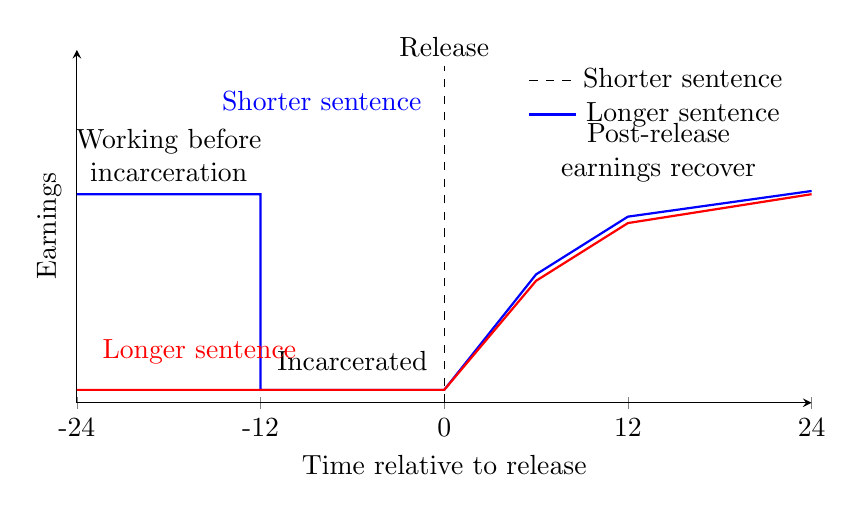
\begin{tikzpicture}
\begin{axis}[
    width=0.9\textwidth,
    height=0.5\textwidth,
    xmin=-24, xmax=24,
    ymin=0, ymax=11,
    axis lines=left,
    xlabel={Time relative to release},
    ylabel={Earnings},
    xtick={-24,-12,0,12,24},
    xticklabels={-24,-12,0,12,24},
    ytick=\empty,
    clip=false,
    legend style={
        at={(0.98,0.98)},
        anchor=north east,
        draw=none,
        fill=none
    }
]

% vertical line at release
\addplot[dashed, black] coordinates {(0,0) (0,10.5)};
\node[above] at (axis cs:0,10.5) {Release};

% shorter sentence: earnings, then incarceration, then recovery
\addplot[thick, blue] coordinates {
    (-24,6.5)
    (-12,6.5)
    (-12,0.4)
    (0,0.4)
    (6,4.0)
    (12,5.8)
    (24,6.6)
};

% longer sentence: longer period of zero earnings, then similar recovery
\addplot[thick, red] coordinates {
    (-24,0.4)
    (0,0.4)
    (6,3.8)
    (12,5.6)
    (24,6.5)
};

% labels
\legend{Shorter sentence, Longer sentence}

% annotations
\node[align=center] at (axis cs:-18,7.7) {Working before\\incarceration};
\node[align=center] at (axis cs:-6,1.3) {Incarcerated};
\node[align=center] at (axis cs:14,7.8) {Post-release\\earnings recover};

% brace-like text labels
\node[align=center, blue] at (axis cs:-8,9.4) {Shorter sentence};
\node[align=center, red] at (axis cs:-16,1.6) {Longer sentence};

\end{axis}
\end{tikzpicture}
\caption{Conceptual earnings paths for individuals with shorter and longer incarceration spells, aligned by release date. The longer-sentence individual loses more earnings during incarceration, but post-release earnings paths may converge.}
\label{fig:qualitative_release_earnings}
\end{figure}
}
\vspace{10cm}


\item Table \ref{fig:kling_table} reports OLS and instrumental
variables (IV) estimates from Kling (2006) of the effect of
an additional year of incarceration on labor market outcomes
nine years after incarceration began.

\begin{figure}[h!]
\centering
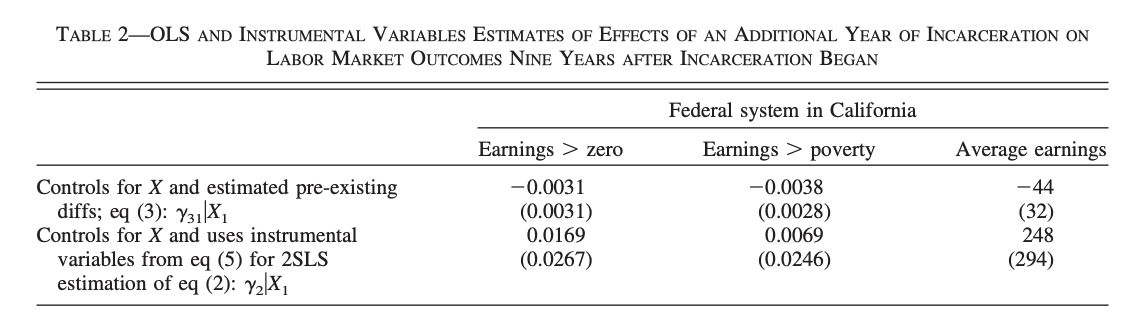
\includegraphics[width=0.95\textwidth]{table1.png}
\caption{Kling (2006), Table 2.}
\label{fig:kling_table}
\end{figure}

\begin{enumerate}[label=(\alph*)]
\item Interpret the OLS estimates for ``Earnings $>$ zero''
and ``Average earnings.'' What do their signs and
magnitudes suggest?
% SOLUTION:
% The OLS estimate for Earnings > zero is -0.0031, meaning
% that an additional year of incarceration is associated
% with a 0.31 percentage point lower probability of
% having positive earnings nine years after incarceration began.
% The average earnings coefficient is -44, meaning an
% additional year is associated with $44 lower average earnings
% (in the outcome's reported monetary units).
% Neither estimate is statistically significant.
\vspace{3cm}

\item Comment on the sign of the OLS estimate relative to the IV estimate for both outcomes. 
% SOLUTION:
% Individuals who receive longer sentences may differ
% systematically from those receiving shorter sentences.
% For example, defendants with more serious offenses,
% more extensive criminal histories, or weaker prior
% labor market attachment may receive longer sentences
% and also have worse future employment outcomes.
% This creates downward bias in the OLS estimates,
% potentially making incarceration appear more harmful.
% IV exploits judge-induced variation in sentence length
% to address this endogeneity, under the IV assumptions.
% However, a sign reversal alone does not prove that
% selection bias explains the difference: the estimates
% may also differ because of sampling variation or
% because IV identifies a different causal effect.
\vspace{2.5cm}

\item Interpret the IV estimate of 0.0169 for
``Earnings $>$ zero.'' What population does this
estimate apply to?
% SOLUTION:
% The IV point estimate suggests that an additional
% year of incarceration increases the probability
% of having positive earnings by 1.69 percentage points.
% Under the identifying assumptions, this is a local
% causal effect for individuals whose sentence lengths
% are changed by the instrument, rather than necessarily
% the average effect for all incarcerated individuals.
% The estimate is not statistically significant.
\vspace{2cm}

\item Can we conclude from this table that longer
incarceration increases employment and earnings?

% SOLUTION:
% No. The IV estimates are positive, but none is
% statistically significant at conventional levels.
% For example, the IV coefficient for Earnings > zero
% is 0.0169 with a standard error of 0.0267.
% The approximate 95% confidence interval is
% 0.0169 +/- 1.96(0.0267) = [-0.0354, 0.0692].
% This interval includes zero and both negative and
% positive effects.
% The evidence therefore does not establish that
% longer incarceration improves labor market outcomes.
% Statistical insignificance also does not prove
% that the true causal effect is exactly zero.
\vspace{2cm}
\end{enumerate}


\vspace{1.5cm}

\end{enumerate}

\newpage

% ==========================================================
\section*{Part D. Hjalmarsson et al.\ (2025): Job Sorting And The \mbox{Labor} Market Effects Of A Criminal Record}
% ==========================================================

\noindent\textit{Study:}
Hjalmarsson, Lindquist, Lepage, and Miller use Swedish registers
to compare people \emph{charged for the first time} to matched
people \emph{suspected of similar offenses but not charged}.
They observe work and employers before and after the event.
The paper version estimates that
acquiring a record reduces months employed by about 2\%
and annual earnings by about 5\%.
These are effects of a \emph{record}, not an additional month in prison.

\begin{enumerate}[resume]

\item Why is comparing first-time charged individuals to similarly
suspected but uncharged individuals potentially more informative
than comparing everyone with and without a record?

Name one remaining threat to identification.

\answer{
Both groups experienced police suspicion regarding similar offenses,
which improves comparability and helps account for consequences
of investigation itself.
Remaining concerns include differences in underlying evidence,
offense severity, or concurrent shocks that both determine charging
and change work trajectories.
Matching is not randomized charging.
}
\vspace{3cm}

\item The authors use an event-study-style design.

Suppose $D_i=1$ denotes the first-charge group,
and $t=0$ is the event year.

Consider

\[
Y_{it}
=
\alpha_i+\lambda_t+
\sum_{k\neq -1}
\beta_k D_i\mathbf{1}\{t=k\}
+\varepsilon_{it}.
\]

\begin{enumerate}[label=(\alph*)]

\item What do $\alpha_i$, $\lambda_t$, and $\beta_2$ represent?
Why omit event time $k=-1$?

\answer{
Person fixed effects absorb time-invariant person traits;
year effects absorb common shocks.
$\beta_2$ is the treated-versus-control earnings difference
two event years after the focal event, relative to the gap
in event year $-1$, after the controls.
One event-time coefficient is omitted as the normalization
or reference period.
}
\vspace{3cm}

\item State the key \emph{parallel trends} assumption
in plain language.

What would you look for among the coefficients with $k<0$?
Do similar pre-trends prove the assumption?

\answer{
Absent the first charge or record, the two matched groups'
average labor outcomes would have evolved similarly.
Leads in pre-event years should be near zero, without
systematic trends, though observed pre-trends alone cannot
prove that post-event counterfactual trends would coincide.
}
\vspace{3cm}

\end{enumerate}

\item Write a difference-in-differences equation.

Let $Charged_i$ indicate the first-charge group and $Post_t$
indicate the post-event period.

Write a two-period DiD regression with an intercept,
both main effects, and an interaction.

Which coefficient estimates the DiD effect?
Explain what the identifying assumption requires.

\answer{
A suitable specification is
$Y_{it}=\alpha+\beta Charged_i+\gamma Post_t+
\delta(Charged_i\times Post_t)+u_{it}$.

The interaction coefficient $\delta$ is the DiD contrast.
It is interpreted as causal under parallel trends and no relevant
spillovers or concurrent group-specific shocks.

The counterfactual earnings trend for charged workers must match
the trend for comparison workers absent the charge.
}
\vspace{1.7cm}


\item Figures \ref{fig:record_eventstudy} show event-study
estimates from Hjalmarsson et al. (2025) of the effect of
acquiring a criminal record on employment and earnings.
The omitted reference period is the year immediately before
the suspected offense ($t=-1$). The vertical bars represent
95\% confidence intervals.

\begin{figure}[h!]
\centering
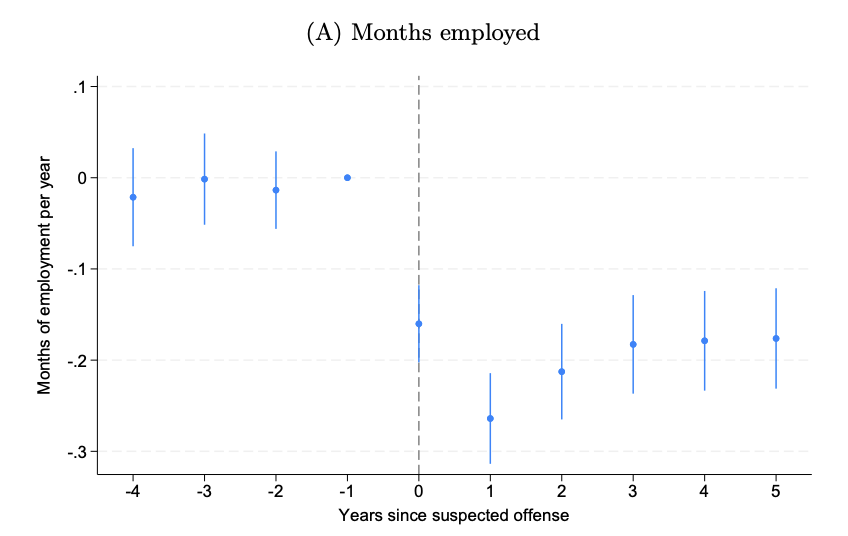
\includegraphics[width=0.75\textwidth]{fig1.png}
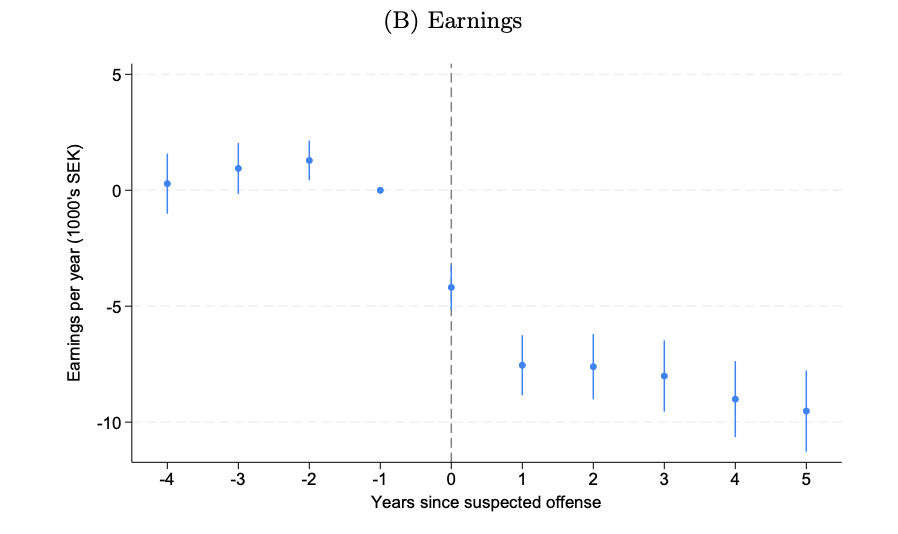
\includegraphics[width=0.75\textwidth]{fig2.png}
\caption{Effects of acquiring a criminal record on employment
and earnings. Source: Hjalmarsson et al. (2025).}
\label{fig:record_eventstudy}
\end{figure}

\begin{enumerate}[label=(\alph*)]

\item Examine the estimates before the suspected offense.
What do these pre-treatment coefficients suggest about
the parallel trends assumption? Does this prove that
the identifying assumption holds?
\vspace{2cm}
% SOLUTION:
% Before the suspected offense, the coefficients are
% generally close to zero, although some earnings
% coefficients are positive.
% This is broadly reassuring for parallel trends,
% but does not prove the identifying assumption.
% Similar observed pre-trends do not guarantee that
% untreated potential outcomes would have evolved
% similarly after the event.

\item Interpret the estimated effects on months employed
and annual earnings one year after the suspected offense.
Be precise about the units.
\vspace{2cm}
% SOLUTION:
% Panel A: At t=1, the estimate is approximately -0.26.
% Acquiring a criminal record reduces employment by
% approximately 0.26 months per year, or about 8 days
% of employment annually, relative to the comparison group.
%
% Panel B: At t=1, the estimate is approximately -7.5.
% Since earnings are measured in thousands of Swedish
% kronor (SEK), this corresponds to about 7,500 SEK
% lower annual earnings.
%
% These are approximate values read from the figures.

\item Are the estimated effects statistically significant
one year after the offense? How can you tell from
the confidence intervals?
\vspace{2cm}
% SOLUTION:
% Yes. At t=1, both confidence intervals lie entirely
% below zero, indicating statistically significant
% negative effects at the 5% level.
% If a 95% confidence interval includes zero, we
% cannot reject a zero effect at the 5% level.


\item Is the pooled average in the post-period statistically significant? How can you tell?
\vspace{2cm}
% SOLUTION:
% Yes. The pooled post-period average is negative and
% its confidence interval lies entirely below zero,
% indicating a statistically significant negative effect
% at the 5% level.
% The formal test is a joint test of the post-event coefficients, which reports an F-statistic and p-value in the paper.


\item Do the effects appear temporary or persistent?
Compare the estimates at $t=1$ and $t=5$.
\vspace{2cm}
% SOLUTION:
% The negative effects persist through five years.
% Employment losses become somewhat smaller,
% changing from approximately -0.26 months at t=1
% to approximately -0.18 months at t=5.
% Earnings losses appear to grow in magnitude,
% from roughly 7,500 SEK at t=1 to about
% 9,500 SEK at t=5.
% These patterns suggest persistent labor market
% consequences of acquiring a criminal record.

\item A student concludes:
``Since earnings fall more than employment, the entire
earnings loss must be caused by lower wages rather than
reduced employment.''

Is this conclusion justified? What additional outcomes
would help distinguish the possible mechanisms?
\vspace{2cm}
% SOLUTION:
% No. Total annual earnings depend on employment duration,
% hours worked, and wages.
% A reduction in earnings could reflect fewer months
% employed, fewer hours conditional on employment,
% lower wages, or sorting into lower-paying firms.
% The two figures alone cannot isolate these channels.
% Useful additional outcomes include hourly wages,
% hours worked, earnings conditional on employment,
% and characteristics of employers before and after
% the event.

\end{enumerate}


\end{enumerate}

% ==========================================================
\section*{Part E. Employer Sorting and Policy}
% ==========================================================

\noindent\textbf{Finding:}
In the paper, workers with records become less likely to work
at firms classified as less willing to hire workers with records,
more likely to work at other firms, and have lower monthly earnings
across firm types.
Firms differ substantially in willingness to employ workers
with records, even within industries.

\begin{enumerate}[resume]

\item Imagine two firms in the same industry.

Firm A pays well but rarely employs people with records;
Firm B regularly hires people with records.

Explain how a new record could lower a worker's earnings
through \emph{sorting} even if the worker stays employed.

Why does the within-firm-type earnings finding matter?

\answer{
A record can restrict access to high-paying employers and shift
a worker toward employers offering lower wages or hours.
But earnings declines within firm types suggest that employer
sorting alone does not fully explain the total earnings penalty.
Other wage, hours, or matching channels also matter.
}
\vspace{1.1cm}

\item Interpret an interaction.

Suppose researchers estimate

\[
\begin{aligned}
Y_{it}={}&
\alpha_i+\lambda_t
+\beta(Charged_i\times Post_t)\\
&+\theta(Charged_i\times Post_t\times HighPay_i)\\
&+\phi(HighPay_i\times Post_t)+\varepsilon_{it},
\end{aligned}
\]

where $HighPay_i$ indicates that a worker's employer
\emph{before the event} was high-paying.

What is the estimated post-event effect for workers at
lower-paying versus higher-paying employers before the event?

What does $\theta$ test?

\answer{
The estimated post-event effect is $\beta$ for $HighPay_i=0$
and $\beta+\theta$ for $HighPay_i=1$.
The coefficient $\theta$ measures the difference between these
two effects, not the overall effect for high-paying-firm workers.

Conditioning on the pre-event employer avoids defining groups
based on an outcome potentially affected by treatment.

This is a hypothetical specification, not the paper's regression.
}


\end{enumerate}


\end{document}
